\documentclass[10.5pt
%,draft
]{article}

\usepackage{CTEX}
\usepackage{graphicx}
\usepackage{amsmath}
\usepackage{natbib}

\begin{document}

\renewcommand{\refname}{参考文献}
\renewcommand{\figurename}{图}
\renewcommand{\abstractname}{摘要}

\title{一维磁流体力学激波--第4次作业\footnote{2019年秋季《磁流体力学的数值模拟方法》}}

\author{
	毛东巍\footnote{邮箱: mdw97@mail.ustc.edu.cn  学号: SA19007035}\quad 
	张建\footnote{邮箱: zj250711@mail.ustc.edu.cn  学号: SA19007060}\quad 
	钟志辉\footnote{邮箱: zzhustc@mail.ustc.edu.cn  学号: SA19007054}
}

\date{%
\scriptsize%
%CAS Key Laboratory for Basic Plasma Physics, School of Earth and Space Sciences,
%\\
%University of Science and Technology of China, Hefei, Anhui 230026, China
中国科学院近地空间环境重点实验室, 合肥 230026\\
中国科学技术大学地球与空间科学学院, 合肥 230026
%
}

\maketitle

\begin{abstract}
讨论了一维磁流体力学(MHD)激波问题的有限差分数值解法, 结合理论分析讨论了磁声波的特性,
分析了数值格式的计算效果.
\end{abstract}

\section{一维磁流体力学激波\citep{Jeffrey1964}}
守恒型方程
\begin{align}
\frac{\partial U}{\partial t} + \nabla \cdot \boldsymbol{F} = 0. \label{Eqn:3.1.6}
\end{align}

对一维磁流体, 设所有的物理量只是$x$和$t$的函数,
\begin{align}
U_t + F_x = 0\label{Eqn:6.1.1}
\end{align}

本文使用了无量纲数值, 可以将磁流体力学方程表示为
\begin{align}
\frac{\partial U}{\partial t} + \frac{\partial F}{\partial x} = 0 \label{Eqn:MHD}
\end{align}
其中
\begin{align}
U = & \left[ \begin{array}{l}
\rho\\
\rho v^2 + H_y^2 + H_z^2 + \frac{\beta p}{\gamma -1}
\\
\rho v_x\\
\rho v_y\\
\rho v_z\\
H_y\\
H_z
\end{array} \right], \label{Eqn:U}\\
F = & \left[ \begin{array}{l}
\rho v_x\\
\rho v_x \left(v^2 + \frac{\gamma}{\gamma - 1} \frac{\beta p}{\rho} \right) + 2(H_y^2 v_x + H_z^2 v_x - H_x H_y v_y - H_x H_z v_z)
\\
\rho v_x^2 + \frac{\beta}{2} p + \frac{1}{2} (H_y^2 + H_z^2)\\
\rho v_x v_y - H_x H_y\\
\rho v_x v_z - H_x H_z\\
v_x H_y - v_y H_x\\
v_x H_z - v_z H_x
\end{array} \right] \label{Eqn:Flux}
\end{align}
这里$v^2 = v_x^2 + v_y^2 + v_z^2$. 若取$\rho_0 = 1$, $p_0 = 1$, $v_0 = 1$, $H_0 = 1/\sqrt{4\pi}$, 则$\beta = 2$.

\section{数值实验}

考虑下列初值问题
\begin{align}
U(x,t)|_{t=0} = \left\{ \begin{array}{ll}
U_L, & \quad x < x_0 \\
U_R, & \quad x > x_0
\end{array} \right.
\end{align}
或者
\begin{align}
W(x,t)|_{t=0} = \left\{ \begin{array}{ll}
W_L, & \quad x < x_0 \\
W_R, & \quad x > x_0
\end{array} \right.
\end{align}
的有限差分数值计算. 这里$U$表达式由方程(\ref{Eqn:U})给出, 而
\begin{align}
W = \left[ \begin{array}{ccccccc}
\rho,
p,
v_x,
v_y,
v_z,
H_y,
H_z
\end{array} \right]^T.
\end{align}
上标$T$表示转置操作. 取$\gamma=5/3$, $\mu=1$, $H_x=5$. 对下面两种初值条件,
利用Lax-Wendroff格式\citep{Zheng2019}
\begin{align}
\left\{\begin{array}{ll}{U_{j+1 / 2}^{n+1 / 2}=\frac{1}{2}\left(U_{j}^{n}+U_{j+1}^{n}\right)-\frac{\Delta t}{2\Delta x}\left(F_{t+1 / 2}^{n}-F_{j}^{n}\right)} \\ {U_{j}^{n+1}=U_{j}^{n}-\frac{\Delta t}{\Delta x}\left(F_{j+1 / 2}^{n+1 / 2}-F_{j-1 / 2}^{n+1 / 2}\right)}\end{array}\right.
\end{align}
进行数值求解并作图讨论结果.

\subsection{较弱的快激波}
取$x_0 = 0.0$, 快激波条件为
\begin{align}
W_L =& \left[\begin{array}{cccccc}
2.121,
4.981,
-13.27,
-0.163,
-0.6521,
2.572,
10.29
\end{array}\right]^T,
\nonumber\\
W_R =& \left[\begin{array}{ccccccc}
1,
1,
-15.3,
0,
0,
1,
4
\end{array}\right]^T. \label{Eqn:WFast}
\end{align}
其中快激波的计算结果如图\ref{Fig:WFast}所示.
\begin{figure}[htb]
\begin{center}
\begin{tabular}{cc}
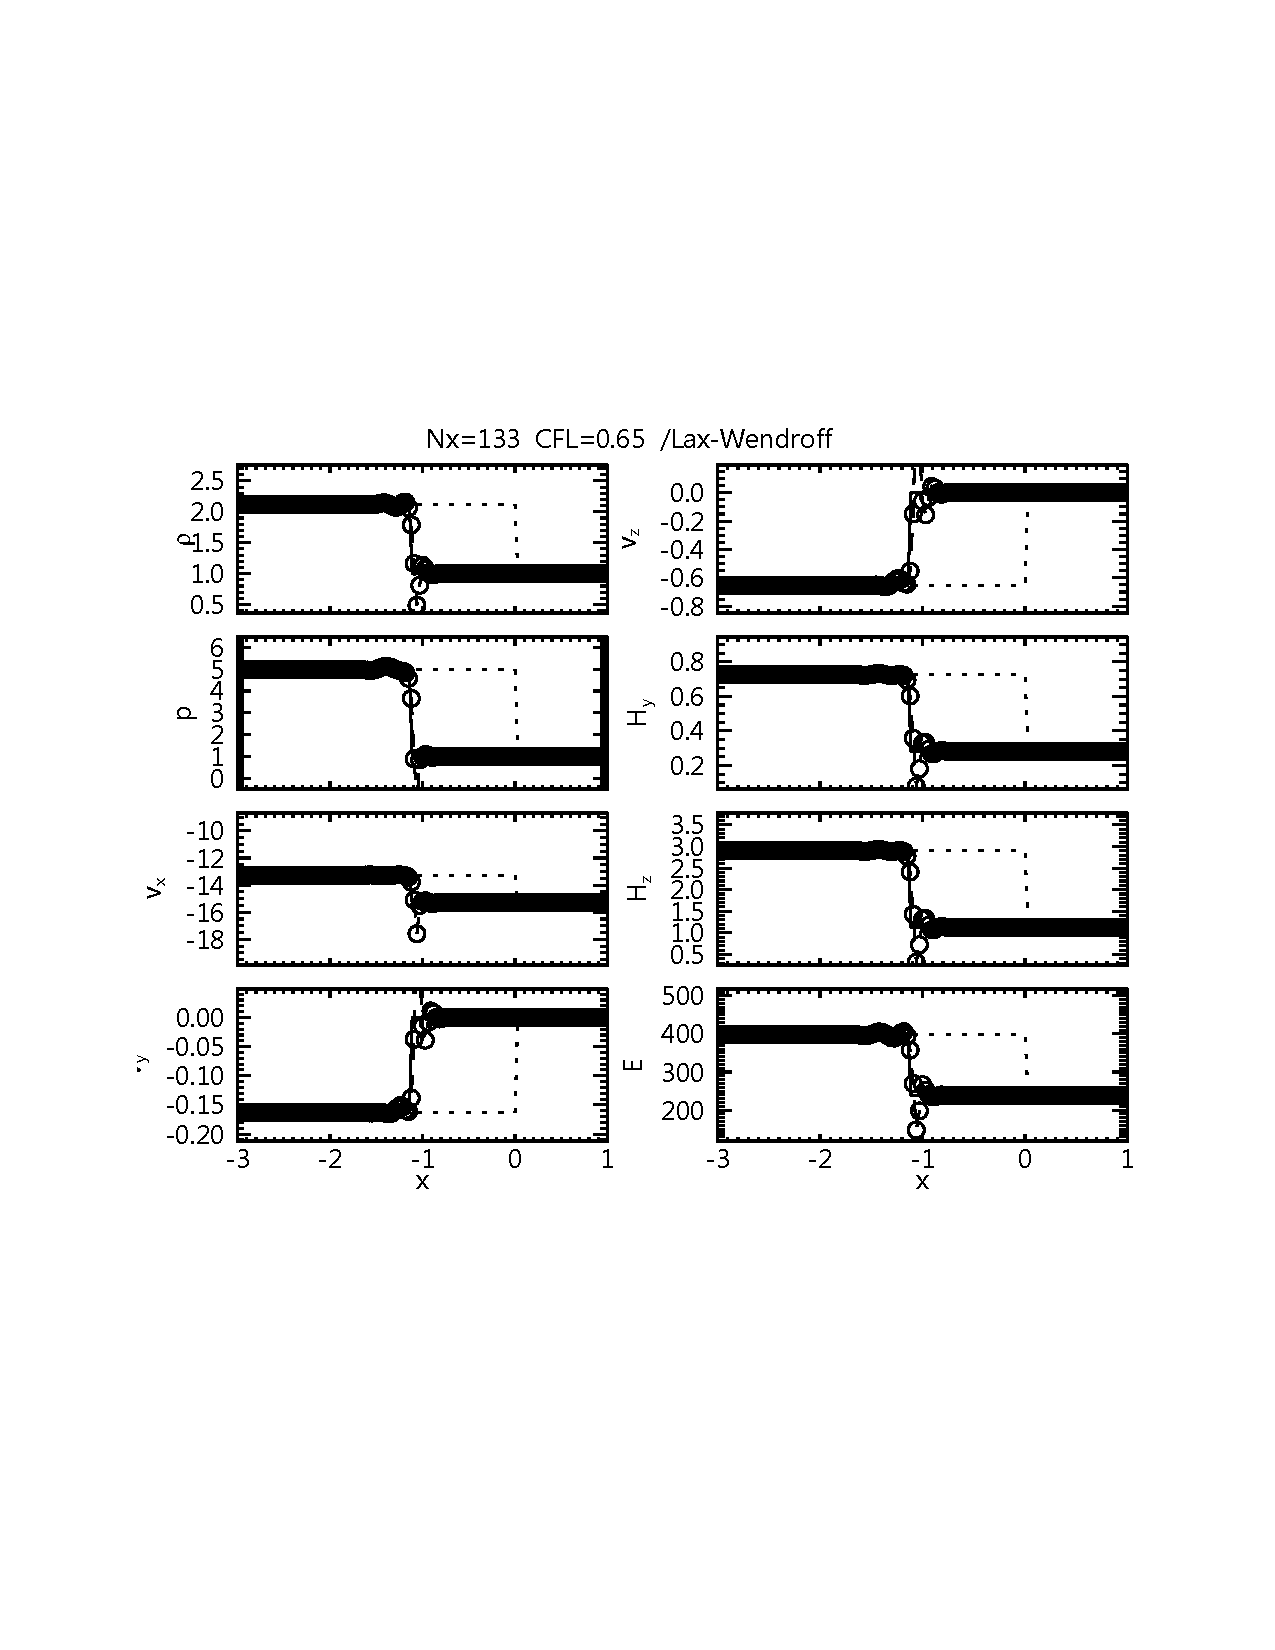
\includegraphics[width=.45\textwidth]{hw4_lw_1f1.pdf}&
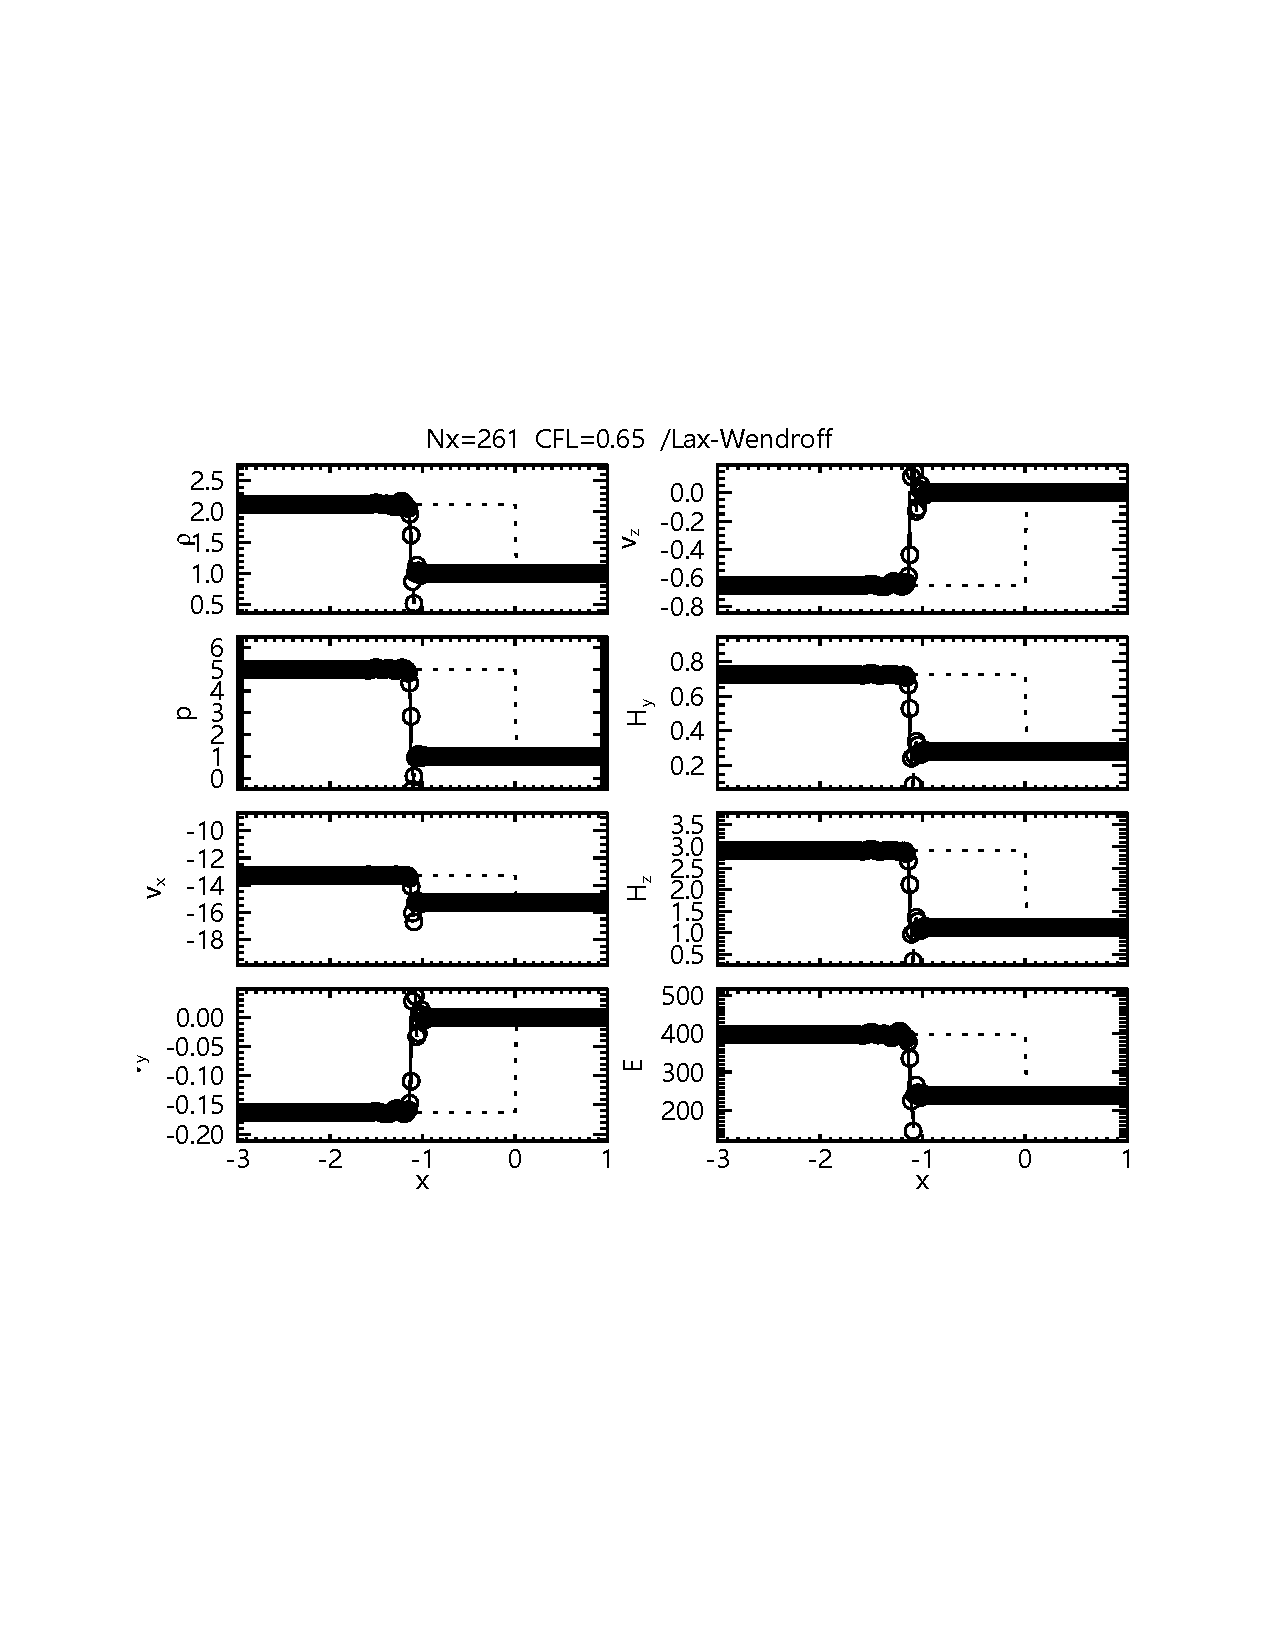
\includegraphics[width=.45\textwidth]{hw4_lw_1f2.pdf}
\\
(a)&(b)
\end{tabular}
\caption{初值条件 (\ref{Eqn:WFast}) 情况下的快激波在$t = 0.1$时的Lax-Wendroff格式计算结果. 数据为无量纲形式的密度, 压强, 速度, 磁场和能量. 图中$\circ$为数值解的数据点, 虚线为数值解, 点线为初始值, 实线为解析解. (a) 网格数为133; (b) 网格数为261.} \label{Fig:WFast}
\end{center}
\end{figure}

\subsection{一维MHD快激波(Mach数为10)\citep{Dai1994}}
取$x_0 = 0.2$, 快磁声激波的初值条件为
\begin{align}
W_L =& \left[\begin{array}{cccccc}
3.896,
305.9,
0,
-0.058,
-0.226,
3.951,
15.8
\end{array}\right]^T,
\nonumber\\
W_R =& \left[\begin{array}{ccccccc}
1,
1,
-15.3,
0,
0,
1,
4
\end{array}\right]^T.\label{Eqn:Fast}
\end{align}
使用Lax-Wendroff格式的数值计算结果如图\ref{Fig:Fast}所示.
\begin{figure}[htb]
\begin{center}
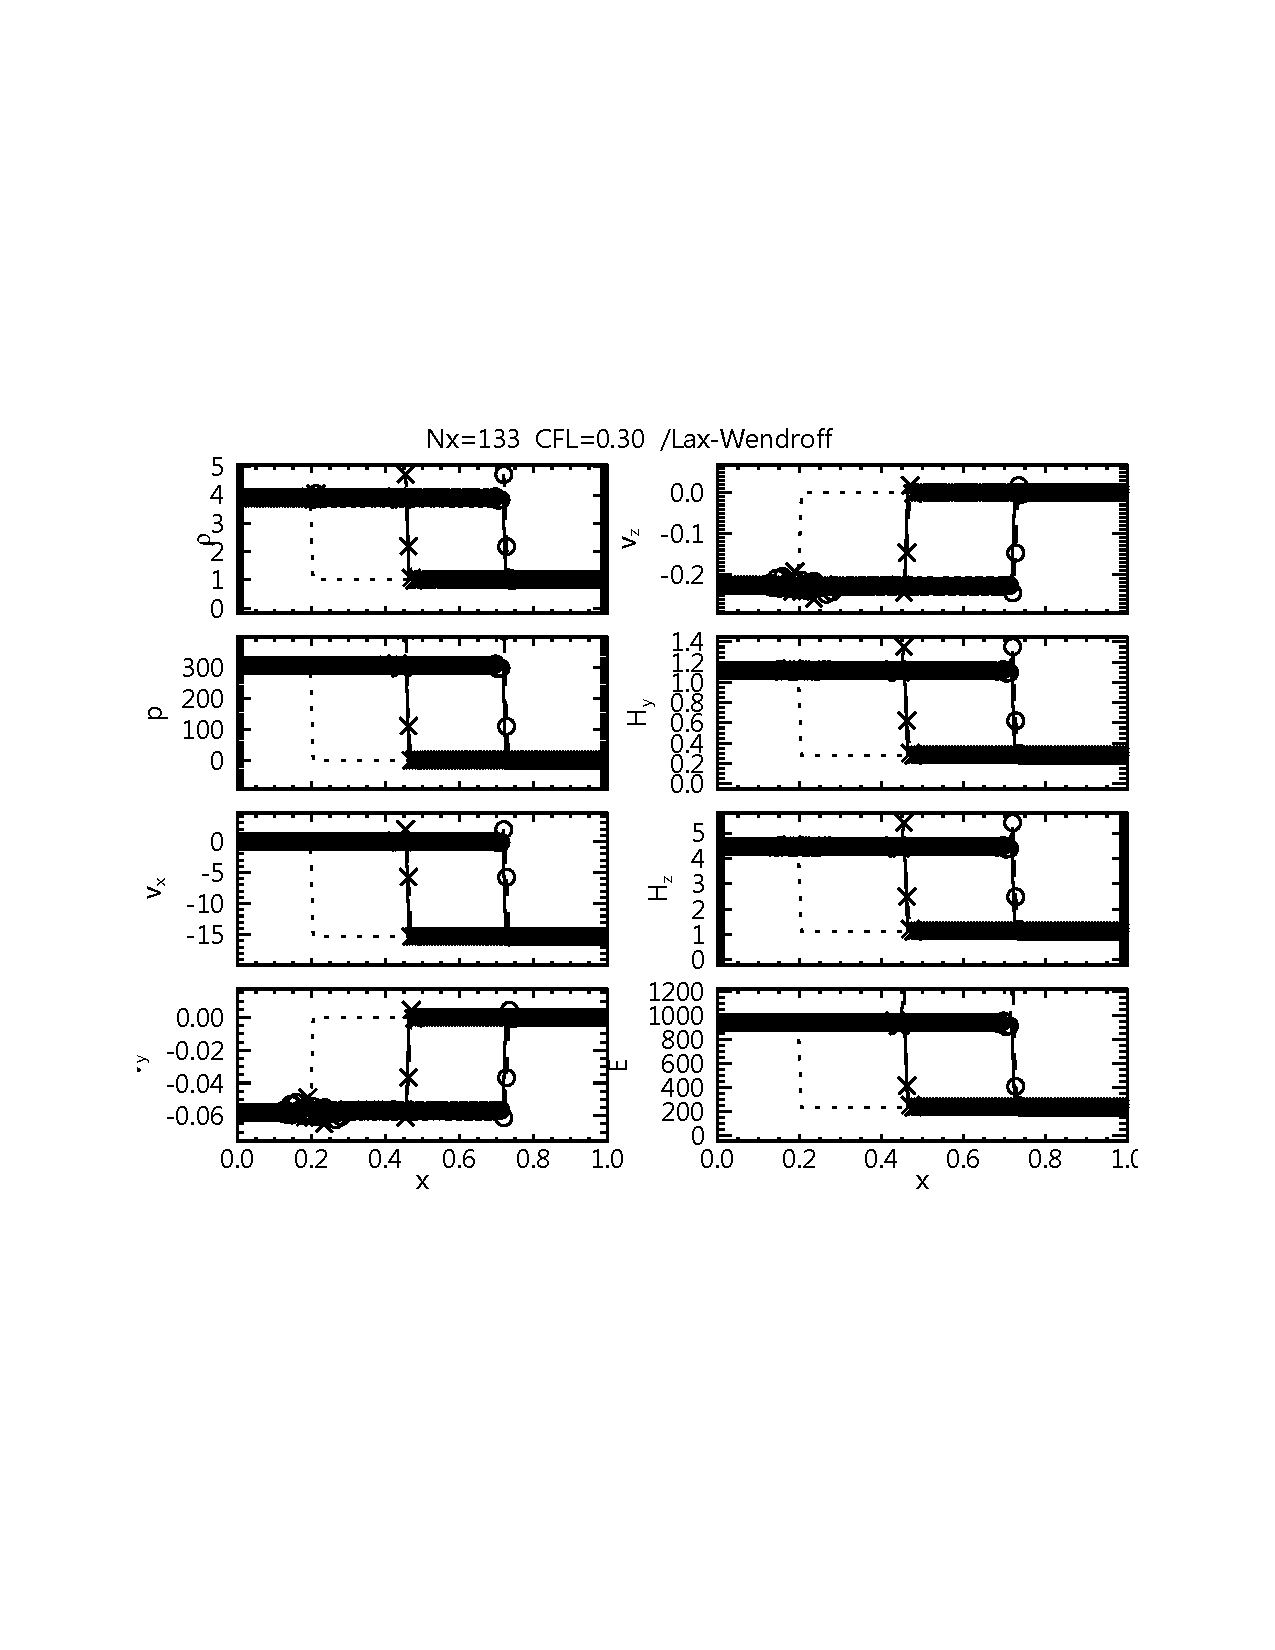
\includegraphics[height=.78\textwidth]{hw4_lw_2f.pdf}
\caption{初值条件 (\ref{Eqn:Fast}) 情况下快激波的Lax-Wendroff格式对应于$t=0$, 0.05和0.1时, 网格数为133的计算结果. 图中$\circ$为$t=$0.1, $\times$为$t=$0.05, 其他同图\ref{Fig:WFast}. }\label{Fig:Fast}
\end{center}
\end{figure}

\subsection{一维MHD慢激波(Mach数为3.5)\citep{Dai1994}}
同样取$x_0 = 0.2$, 慢磁声激波的初值条件为
\begin{align}
W_L =& \left[\begin{array}{ccccccc}
3.108,
1.4336,
0,
0.2633,
0.2633,
0.1,
0.1
\end{array}\right]^T,
\nonumber\\
W_R =& \left[\begin{array}{ccccccc}
1,
0.1,
-0.9225,
0,
0,
1,
1
\end{array}\right]^T.\label{Eqn:Slow}
\end{align}
使用Lax-Wendroff格式的数值计算结果如图\ref{Fig:Slow}所示.
\begin{figure}[htb]
\begin{center}
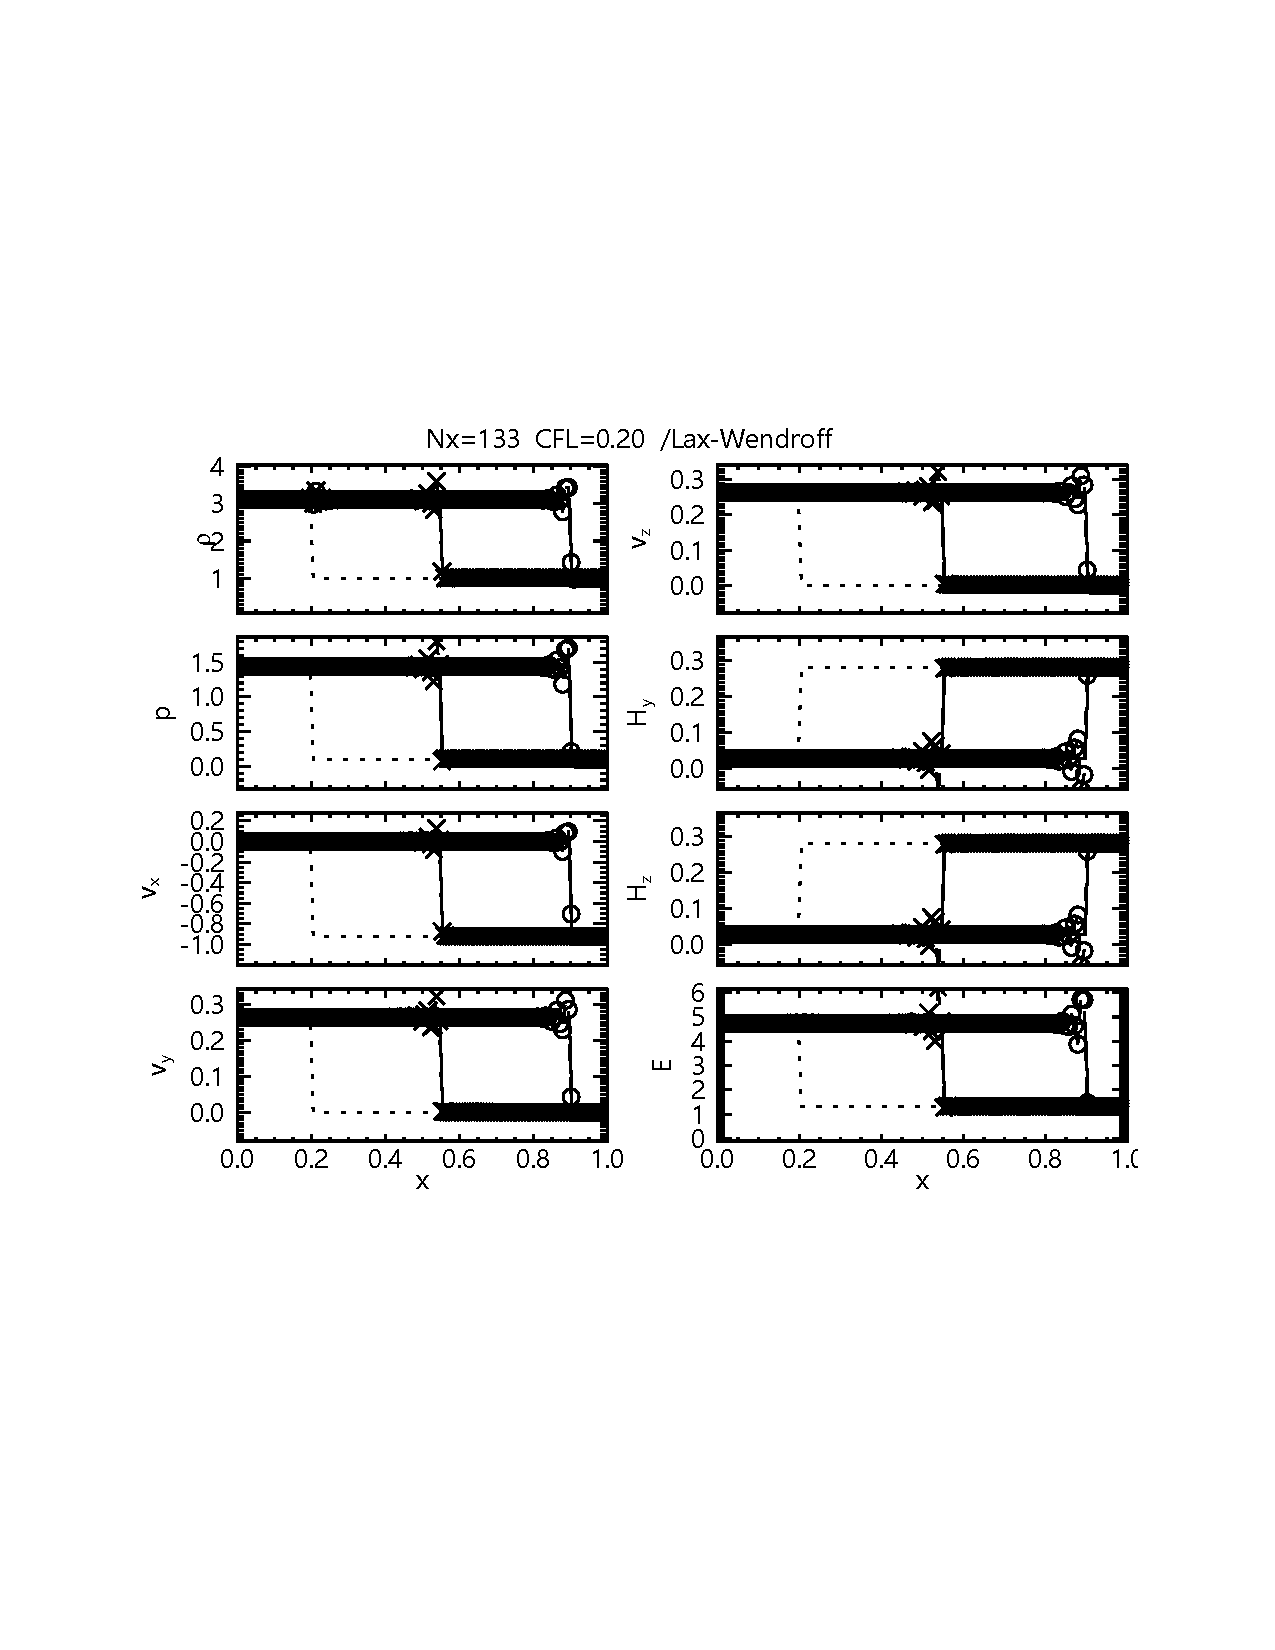
\includegraphics[height=.78\textwidth]{hw4_lw_2s.pdf}
\caption{初值条件 (\ref{Eqn:Slow}) 情况下慢激波的Lax-Wendroff格式对应于$t=0$, 0.8和1.6时, 网格数为133的计算结果. 图中$\circ$为$t=$0.8, $\times$为$t=$1.6, 其他同图\ref{Fig:WFast}. }\label{Fig:Slow}
\end{center}
\end{figure}

\subsection{数值计算结果分析}
从图\ref{Fig:WFast}, 图\ref{Fig:Slow}和图\ref{Fig:Fast}中可以看到, 使用Lax-Wendroff格式进行数值计算会出现上冲和下冲.

\section*{分工说明}

\begin{itemize}
	\item 毛东巍: 完成图\ref{Fig:Slow};
	\item 张建: 完成报告和图\ref{Fig:Fast};
	\item 钟志辉:完成图\ref{Fig:WFast}.
\end{itemize}
特此说明: 以上分工仅以姓名拼音为序.
\section{附件}
\begin{enumerate}
\item
assign4.tex--本报告\LaTeX 源文件
\item
assign4.pdf--本报告PDF输出文件
\item
hw4.pro--本报告IDL程序
\item 
functions\_for4.pro--IDL程序中使用的自定义函数
\item
References.bib -- 文献文件
\item
hw4\_lw\_1f1.pdf--初值条件 (\ref{Eqn:WFast}) 情况下的快激波数值结果 (Lax-Wendroff格式), 133网格
\item
hw4\_lw\_1f2.pdf--初值条件 (\ref{Eqn:WFast}) 情况下的快激波数值结果 (Lax-Wendroff格式), 261网格
\item
hw4\_lw\_2f.pdf--初值条件 (\ref{Eqn:Fast}) 情况下 (快磁声激波) 数值计算得到的物理量各时刻图形 (Lax-Wendroff格式)
\item
hw4\_lw\_2s.pdf--初值条件 (\ref{Eqn:Slow}) 情况下 (慢磁声激波) 数值计算得到的物理量各时刻图形 (Lax-Wendroff格式)
\end{enumerate}

\bibliographystyle{apalike}
\bibliography{References}

\end{document}
